\documentclass[12pt]{article}

\usepackage{amsmath, mathtools}
\usepackage{amsfonts}
\usepackage{amssymb}
\usepackage{graphicx}
\usepackage{colortbl}
\usepackage{xr}
\usepackage{hyperref}
\usepackage{longtable}
\usepackage{xfrac}
\usepackage{tabularx}
\usepackage{float}
\usepackage{siunitx}
\usepackage{booktabs}
\usepackage{caption}
\usepackage{pdflscape}
\usepackage{afterpage}

\usepackage[round]{natbib}

\usepackage{titlesec}

%\usepackage{refcheck}

\hypersetup{
    bookmarks=true,         % show bookmarks bar?
      colorlinks=true,       % false: boxed links; true: colored links
    linkcolor=red,          % color of internal links (change box color with linkbordercolor)
    citecolor=green,        % color of links to bibliography
    filecolor=magenta,      % color of file links
    urlcolor=cyan           % color of external links
}

%% Comments
\usepackage{color}
\newif\ifcomments\commentstrue %displays comments
%\newif\ifcomments\commentsfalse %so that comments do not display
\ifcomments
\newcommand{\authornote}[3]{\textcolor{#1}{[#3 ---#2]}}
\newcommand{\todo}[1]{\textcolor{red}{[TODO: #1]}}
\else
\newcommand{\authornote}[3]{}
\newcommand{\todo}[1]{}
\fi
\newcommand{\wss}[1]{\authornote{blue}{SS}{#1}} 
\newcommand{\plt}[1]{\authornote{magenta}{TPLT}{#1}} %For explanation of the template
\newcommand{\an}[1]{\authornote{cyan}{Author}{#1}}
%% Common Parts
\newcommand{\progname}{4TB6 - Mechatronics Capstone} % PUT YOUR PROGRAM NAME HERE
\newcommand{\authname}{Team \#5, Locked \& Loaded
\\ Abi Nevo, nevoa
\\ Elsa Bassi, bassie
\\ Steffi Ralph, ralphs1
\\ Abdul Iqbal, iqbala18
\\ Stephen De Jong, dejons1
\\ Anthony Shenouda, shenoa2} % AUTHOR NAMES                  

\usepackage{hyperref}
    \hypersetup{colorlinks=true, linkcolor=blue, citecolor=blue, filecolor=blue,
                urlcolor=blue, unicode=false}
    \urlstyle{same}


% For easy change of table widths
\newcommand{\colZwidth}{1.0\textwidth}
\newcommand{\colAwidth}{0.13\textwidth}
\newcommand{\colBwidth}{0.82\textwidth}
\newcommand{\colCwidth}{0.1\textwidth}
\newcommand{\colDwidth}{0.05\textwidth}
\newcommand{\colEwidth}{0.8\textwidth}
\newcommand{\colFwidth}{0.17\textwidth}
\newcommand{\colGwidth}{0.5\textwidth}
\newcommand{\colHwidth}{0.28\textwidth}

% Used so that cross-references have a meaningful prefix
\newcounter{defnum} %Definition Number
\newcommand{\dthedefnum}{GD\thedefnum}
\newcommand{\dref}[1]{GD\ref{#1}}
\newcounter{datadefnum} %Datadefinition Number
\newcommand{\ddthedatadefnum}{DD\thedatadefnum}
\newcommand{\ddref}[1]{DD\ref{#1}}
\newcounter{theorynum} %Theory Number
\newcommand{\tthetheorynum}{T\thetheorynum}
\newcommand{\tref}[1]{T\ref{#1}}
\newcounter{tablenum} %Table Number
\newcommand{\tbthetablenum}{T\thetablenum}
\newcommand{\tbref}[1]{TB\ref{#1}}
\newcounter{assumpnum} %Assumption Number
\newcommand{\atheassumpnum}{P\theassumpnum}
\newcommand{\aref}[1]{A\ref{#1}}
\newcounter{goalnum} %Goal Number
\newcommand{\gthegoalnum}{P\thegoalnum}
\newcommand{\gsref}[1]{GS\ref{#1}}
\newcounter{instnum} %Instance Number
\newcommand{\itheinstnum}{IM\theinstnum}
\newcommand{\iref}[1]{IM\ref{#1}}
\newcounter{reqnum} %Requirement Number
\newcommand{\rthereqnum}{P\thereqnum}
\newcommand{\rref}[1]{R\ref{#1}}
\newcounter{nfrnum} %NFR Number
\newcommand{\rthenfrnum}{NFR\thenfrnum}
\newcommand{\nfrref}[1]{NFR\ref{#1}}
\newcounter{lcnum} %Likely change number
\newcommand{\lthelcnum}{LC\thelcnum}
\newcommand{\lcref}[1]{LC\ref{#1}}
\newcounter{ulcnum} %Unlikely change number
\newcommand{\ltheulcnum}{ULC\theulcnum}
\newcommand{\ulcref}[1]{ULC\ref{#1}}

\usepackage{fullpage}

\newcommand{\deftheory}[9][Not Applicable]
{
\newpage
\noindent \rule{\textwidth}{0.5mm}

\paragraph{RefName: } \textbf{#2} \phantomsection 
\label{#2}

\paragraph{Label:} #3

\noindent \rule{\textwidth}{0.5mm}

\paragraph{Equation:}

#4

\paragraph{Description:}

#5

\paragraph{Notes:}

#6

\paragraph{Source:}

#7

\paragraph{Ref.\ By:}

#8

\paragraph{Preconditions for \hyperref[#2]{#2}:}
\label{#2_precond}

#9

\paragraph{Derivation for \hyperref[#2]{#2}:}
\label{#2_deriv}

#1

\noindent \rule{\textwidth}{0.5mm}

}

%\documentclass{article}


\setcounter{secnumdepth}{4}

\titleformat{\paragraph}
{\normalfont\normalsize\bfseries}{\theparagraph}{1em}{}
\titlespacing*{\paragraph}
{0pt}{3.25ex plus 1ex minus .2ex}{1.5ex plus .2ex}


\begin{document}

\title{Software Requirements Specification for \progname: Smart Bike Lock} 
\author{Abi Nevo\\Elsa Bassi\\Steffi Ralph\\Abdul Iqbal\\Stephen De Jong\\Anthony Shenouda}
\date{\today}
	
\maketitle

~\newpage

\pagenumbering{roman}

\tableofcontents

~\newpage

\section*{Revision History}

\begin{tabularx}{\textwidth}{p{2cm}p{2cm}p{2cm}X}
\toprule {\bf Date} & {\bf Version} & {\bf Name} & {\bf Notes}\\
\midrule
02-10-22 & 1.0 & Elsa & Drafted first draft\\
03-10-22& 1.1 & Stephen & Drafted 1 \& 5, and formatting updates\\
03-10-22 & 1.1 & Abi & Drafted Likely and Unlikely Changes\\
04-10-22& 1.2 & Steffi & Drafted Appendix\\
04-10-22 & 1.3 & Abi & Drafted Dev Plan and added Reflection\\
04-10-22 & 1.3 & Steffi & Added Reflections and Section 3 Removed unnecessary subsections from section4\\
\bottomrule
\end{tabularx}

~\newpage

\section{Reference Material}

This section records information for easy reference.

\subsection{Table of Units}

Throughout this document SI (Syst\`{e}me International d'Unit\'{e}s) is employed
as the unit system.  In addition to the basic units, several derived units are
used as described below.  For each unit, the symbol is given followed by a
description of the unit and the SI name.
~\newline

\renewcommand{\arraystretch}{1.2}
%\begin{table}[ht]
%\begincenter
  \noindent \begin{tabular}{l l l} 
    \toprule		
    \textbf{symbol} & \textbf{unit} & \textbf{SI}\\
    \midrule 
    \si{\metre} & length & metre\\
    \si{\kilogram} & mass	& kilogram\\
    \si{\second} & time & second\\
    \si{\joule} & energy & joule\\
    P or \si{\watt} & power & watt (W = \si{\joule\per\second})\\
    \si{\ampere} or I& current & ampere\\
    \si{\ohm} or R& resistance & ohm\\
    \si{\volt} & voltage & volt\\
    \si{\newton} & force & newton\\
    \si{\newton}M & torque & newton meter\\
    \bottomrule
  \end{tabular}
  %	\caption{Provide a caption}
%\end{table}

\subsection{Table of Symbols}

The table that follows summarizes the symbols used in this document along with
their units.  The choice of symbols was made to be consistent with the heat
transfer literature and with existing documentation for solar water heating
systems.  The symbols are listed in alphabetical order.

\renewcommand{\arraystretch}{1.2}
%\noindent \begin{tabularx}{1.0\textwidth}{l l X}
\noindent \begin{longtable*}{l l p{12cm}} \toprule
\textbf{symbol} & \textbf{unit} & \textbf{description}\\
\midrule 
$B_L$ & hour & battery lifein hours\\
$B_C$ & mAH & battery capacity in amp hours\\
$L_C$ & A/actuation & current drawn per motor actuation\\
$A_\text{num}$ & actuation/charge & number of actuations per charge\\ 
\bottomrule
\end{longtable*}


\subsection{Abbreviations and Acronyms}

\renewcommand{\arraystretch}{1.2}
\begin{tabular}{l l} 
  \toprule		
  \textbf{symbol} & \textbf{description}\\
  \midrule 
  SRS & Software Requirements Specification\\
  \bottomrule
\end{tabular}\\


%\subsection{Mathematical Notation}

\pagenumbering{arabic}


\section{Introduction}

The purpose of the SmartLock project is to design and build a product that will provide bicycle users with a safer, easier, and more accessible way to secure their bike through their smartphone. Additionally, it will provide users with a GPS feature to locate the lock in case of bike theft or misplacement.  It will consist of a physical lock that mounts to a bike and a smartphone application that will function as the user interface through which the lock can be engaged and disengaged wirelessly, as well as located. The project will provide an engineering solution using wireless communication, mechanical design, and smartphone application development. More broadly, it seeks to encourage members of society to pursue biking, in both a transportation and recreational capacity, improving the health of society’s citizens and its environment.  

\subsection{Purpose of Document}

The Requirements Documentation seeks to provide a complete overview of the requirements of the Smart Lock system so as to define the project. The assumptions, inputs and outputs will also be defined in order to outline the problem. Several models will be developed and lastly, likely and unlikely changes will be described. This will communicate a unified and documented plan for the project that can be used after the design stage to verify its functionality and provide an important benchmark. 

\subsection{Scope of Requirements} 

The SmartLock project will build off existing designs to tie together principles of wireless communication, GPS, a mechanical locking mechanism, electrical actuation, and smartphone application development. The system will provide all functions necessary for effective and secure locking and location.  

The SmartLock project will be designed to perform the following functions for the user.  

\begin{enumerate}
\item Wireless communication from the smartphone to the lock and vice versa. 
\item Display of lock and battery status information on the app. 
\item Display of location on the app. 
\item Store and use a replaceable battery. 
\item House a mechanical lock frame. 
\item Perform electrical engagement/disengagement of a locking mechanism. 
\item Be waterproof. 
\end{enumerate}

Not included in the project scope will be Bluetooth wireless connective capabilities, a fully autonomous locking mechanism (one that will both open/close and engage/disengage the lock wirelessly) and a rechargeable battery. We will also be ignoring extreme weather and temperature conditions and their impact on the material properties.

\subsection{Characteristics of Intended Reader} \label{sec_IntendedReader}

The reader will have basic knowledge of how bikes are secured in public settings, namely using mechanical locks and keys or combination locks. They will understand why bike locking is necessary and what it means for a bike to be vulnerable to theft, i.e. that all main parts of the bike must be secured including the frame and wheels. They will also have basic knowledge of wireless communications that can be accessed through smartphone applications. Lastly, the reader will have a high-school level understanding of kinematic and electronics-related physics and math such that they can grasp the mechanical and electrical functionality of the system.  

\subsection{Organization of Document}

The document will follow the base template provided by the Capstone 4TB6 course GitLab. It will be organized with an increasing order of specificity, beginning with the General System Description which will include an overview of the Smart Lock project. The Specific System Description will make up the bulk of the document, describing the project in greater detail with its assumptions, inputs and outputs, goals and models. Finally, since the context of the project is previously stated, the Functional and Non-Functional Requirements will be outlined, as well as any foreseen Likely and Unlikely Changes to the project. Lastly, the Traceability Matrix is included to define the relationships between various relevant formulas, sections and information in the document and how they are used to build the project.  

~\newpage

\section{General System Description}

This section provides general information about the system.  It identifies the
interfaces between the system and its environment describes the user
characteristics and lists the system constraints.  


\subsection{System Context}

 \begin{figure}[h!]
 \begin{center}
 %\rotatebox{-90}
 {
  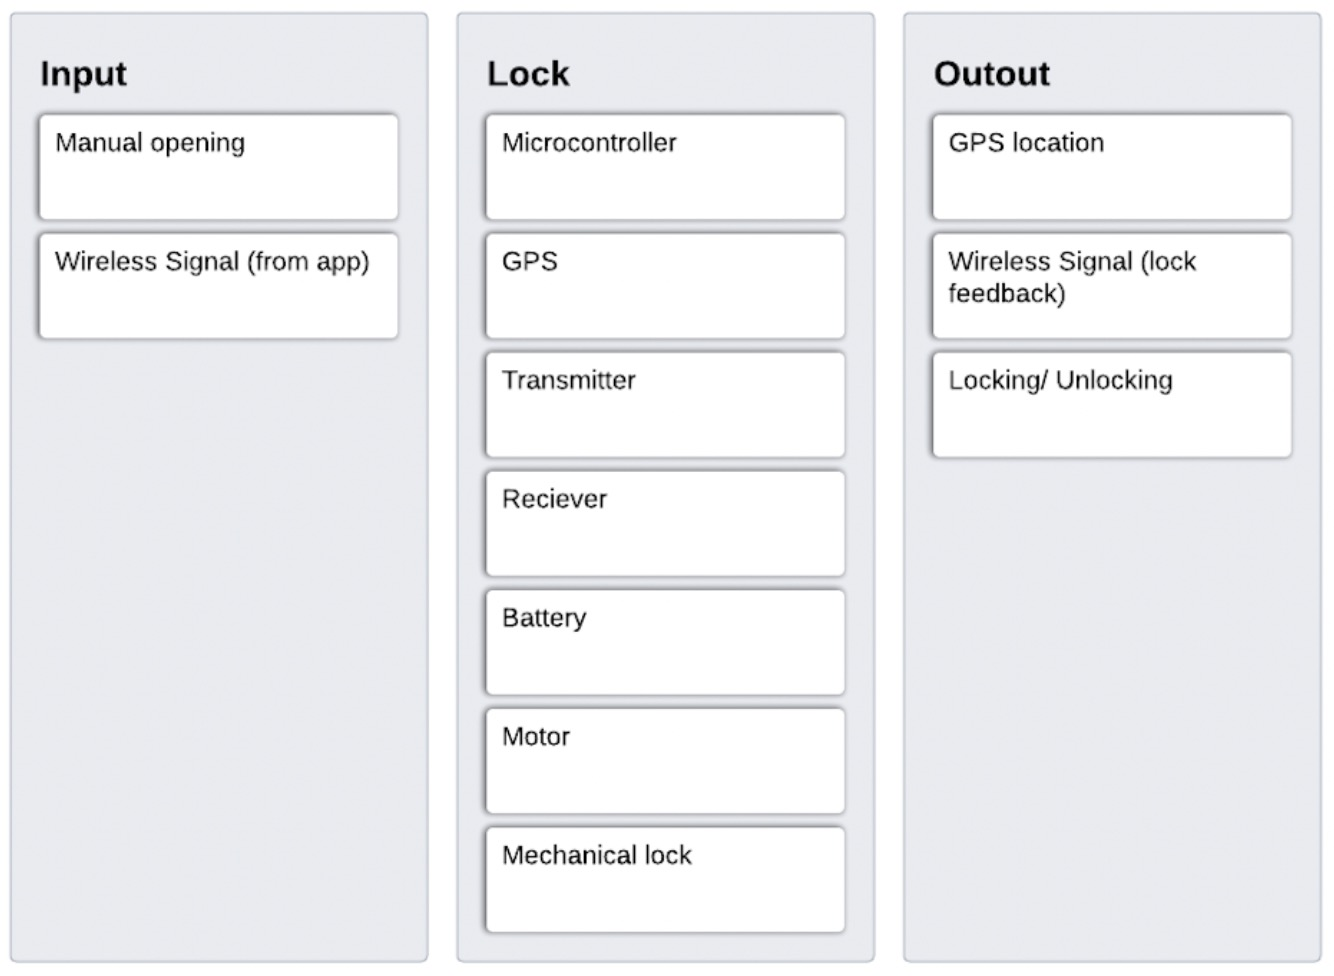
\includegraphics[width=0.6\linewidth]{../SystemContextDiagram.jpeg}
 }
 \caption{\label{The System Context}The System Context: Shows the inputs, the entities that manipulate them, and the outputs.}
 \end{center}
 \end{figure}

\begin{itemize}
\item User Responsibilities:
\begin{itemize}
\item Opening and Closing the physical mechanism
\item Keeping their smartphone with them and charged to be able to use the application
\item Disengaging the lock with their smartphone
\item Leaving their bike in a location where it is possible to connect to an external frame
\end{itemize}
\item \progname{} Responsibilities:
\begin{itemize}
\item Develop a mechanism(s) that closes around the wheels and connects to an external frame
\item Developing a functional lock so that users can feel secure in leaving their bike
\item Developing an app that is user-friendly that disengages the lock and stores the location of the locked bike
\end{itemize}
\end{itemize}

\subsection{User Characteristics} \label{SecUserCharacteristics}


The user of the SmartLock is anyone who owns a bike and a smartphone of any age, gender or biking ability.  The locking mechanism of the SmartLock functions similarly to that of any other locking device, so that no special skills are required to perform the engagement/disengagement of the lock.  The physical mechanism is designed to be simple so that anyone who has the dexterity and physical strength to ride a bike will have the capability to open and close it with no strain.  The application needs to be on a smartphone that supports Bluetooth v4.0 or higher (ie. any iPhone 4S or newer or any Android with OS 4.3 or newer), the user will be expected to understand how basic applications work on these devices.  However, the application itself will be designed to be user-friendly and simple so that the functionality is clear and users do not have to spend lots of time learning the app, and so that the use time of the app when locking your bike is short. 

\subsection{System Constraints}

The system has the following constraints.

\begin{itemize}

\item Locate the bike within a tolerance of 50 meters.
	\begin{itemize}
		\item Justification: Complex software like Google Maps ensures accuracy of around 20 meters. Considering users only require the general location and our software will not be as complex as Google’s, the team added this constraint. 
	\end{itemize}
%Source: https://support.google.com/maps/answer/2839911?hl=en\&co=GENIE.Platform\%3DAndroid 

\item Total mass of lock under 3 lbs. 
	\begin{itemize} 
		\item Justification: Average weight of a bike lock is just under 3 pounds. To ensure the lock was not significantly heavier than average the team added this constraint.
	\end{itemize}
%Source: https://www.nytimes.com/wirecutter/reviews/best-bike-lock/ 

\item App storage under 50 megabytes. 
	\begin{itemize} 
		\item Justification: A small mobile app should not take significant space on the user's phone. Similar GPS applications are around 50 megabytes.
	\end{itemize}
%Source: https://apps.apple.com/us/app/gps-fields-area-measure/id1123033235 

\item The budget for testing, designing, and equipment is \$750.
	\begin{itemize}
		\item Justification: SmartLock has a limited budget to work within to encourage efficient use of materials and ensure low costs.
	\end{itemize} 

\end{itemize}

\subsection{Normal Use Cases}
In general, for a normal use case, the SmartLock system must be able to engage/disengage the SmartLock remotely through the SmartLock mobile interface after which the user must be able to open/close the SmartLock.  The SmartLock must also be able to send "bike parked” location coordinates as well as current SmartLock statuses back to the mobile application. 
\subsubsection{Lock is Engaged/Disengaged}
The lock is to be engaged/disengaged through the SmartLock mobile application.  Given that the user is within range of the system, the SmartLock is designed to receive the corresponding signal request from the user’s smartphone and perform the corresponding action of engaging/disengaging the lock.  The system then sends the current engaged/disengaged status to the mobile application for the user to view.
\subsubsection{Lock is Open/Closed}
Once the request to engage/disengage the lock is sent, the system is not designed to perform the swing action of the lock.  The system is designed to accept the user’s manual input of swinging the lock to the desired open/closed position.  The system then sends the current open/closed status to the mobile application for the user to view. 
\subsubsection{SmartLock location is requested}
The user’s smartphone's current coordinates can be requested through the mobile application by the user.  When the user is near the lock, then they can tag their coordinates, for later use if they forget where their bike is locked.  

\section{Specific System Description}


\subsection{Problem Description} \label{Sec_pd}

There are many problems associated with bike locks today.  People often forget or lose their keys, lock or combination.  Additionally, current locking systems are often not comprehensive – they may not lock all parts of the bike that can be stolen, namely the seat, front and back wheels, and frame.  


Furthermore, bike locks can be bulky, heavy and dangerous to carry around. It can also be tedious to find and lock one’s bike to an external frame.  The combination of these nuisances can lead to individuals leaving their bikes without properly securing them.  The city of Toronto reports an average 3625 stolen bikes annually, and the Canadian Cycling Magazine estimates that only 15-20\% of stolen bikes are reported, which indicates a rather expansive problem that can be solved [1,2].  

\subsubsection{Terminology and  Definitions}

The terms listed below will be used throughout the scope of this document and should be referenced when referring to specific components.  

\begin{itemize}
\item Smart Lock: The scope of this project and document referring to both the mechanical lock and the mobile application communicating with it. 
\item Lock: The physical component of the Smart Lock; includes the hardware, battery, motor, and locking mechanism.  
\item Team: Refers to the members working on Smart Lock 
\item App: The mobile application used to communicate with the lock 
\item Open/Close: The process of physically moving the lock frame into a state where it can be latched onto something else. 
\item Open/Close Status: The current state of the lock frame. 
\item Engage/Disengage: The automated process to actuate the lock to secure the frame. 
\item Wireless Signalling: The means of communication between the lock and the mobile application. 
\item Battery: The power source used to power the motor for engaging and disengaging. 
\item Battery Status: A measure of the quantity of charge in the battery. 
\item Git: The platform used to store the documentation and software and track changes made to the files. 
\item XCode and Flutter: The IDE used to develop the mobile application. 
\item Cross-Platform Development: The means of developing the mobile application on both iOS and Android devices. 
\item Transmitter: The device used to send signals to and from the app to give status information and to send the engagement and disengagement signals. 
\item GPS: The satellite-based navigation system used to locate the bike. 
\item Receiver: The device used to receive the signals from the app for engagement and disengagement. 
\item Microcontroller: The programmable device used to control the motor. 
\end{itemize}
~\newpage
\subsubsection{Physical System Description} \label{sec_phySystDescrip}
~\newline
 \begin{figure}[h!]
 \begin{center}
 %\rotatebox{-90}
 {
 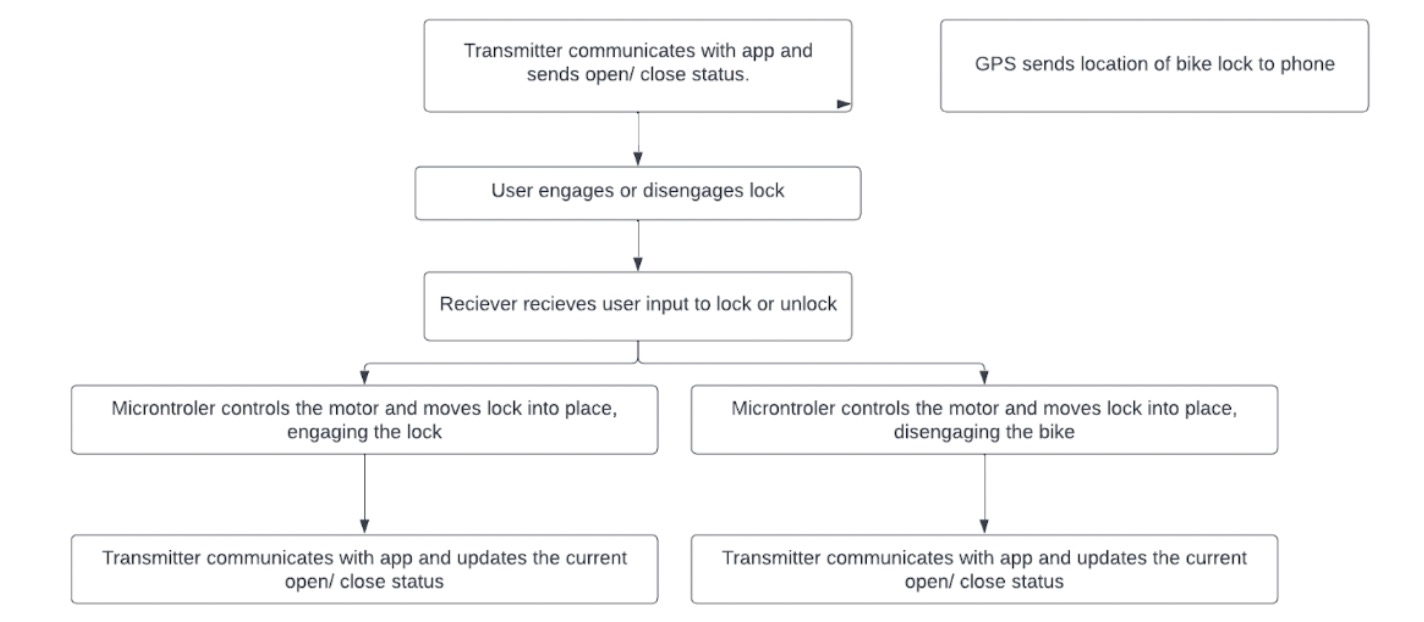
\includegraphics[width=0.6\linewidth]{../FunctionalDiagram.jpeg}
 }
 \caption{\label{The Physical System} The Physical System}
 \end{center}
 \end{figure}

\subsubsection{Goal Statements}



\noindent Given the \plt{inputs}, the goal statements are:

\begin{itemize}

\item[GS\refstepcounter{goalnum}\thegoalnum :] Effective Bike Lock: The lock is sturdy and cannot be manual opened by the average human once engaged.

\item[GS\refstepcounter{goalnum}\thegoalnum :] Long Lasting Battery Life: The power source is used efficiently to last a sufficient period of time without requiring replacement. 

\item[GS\refstepcounter{goalnum}\thegoalnum :] Bicycle Versatility: The lock can be used on mountain, city, kids, and road bikes.

\item[GS\refstepcounter{goalnum}\thegoalnum :] Easily Mountable on Bike Frame: Does not require special tools to be installed. 

\item[GS\refstepcounter{goalnum}\thegoalnum :] Effective GPS Tracking: The lock can accurately transmit location to app regardless of location.  

\item[GS\refstepcounter{goalnum}\thegoalnum :] Weatherproof: The lock is not easily damaged by wind, rain, snow, heat, and cold weather.

\end{itemize}

\subsubsection{Assumptions} \label{sec_assumpt}

\begin{itemize}

\item The bike will be left in locations with strong GPS signal.
Dependencies: Locations such as garages and underground parking. 
\item The user’s phone will always be able to connect to the lock (wireless connection works as intended).
Dependencies: All users have modern phones that can operate the application. The phones will also have functional location settings.  
\item Users will have no limiting physical disabilities.
Dependencies: Average person is strong enough to manually lock and unlock the bike.
\item The lock will be weatherproof.
Dependencies: Rain, snow or extreme temperatures will not damage the lock. 
\item Battery life is only reduced when the motor is being used.
Dependencies: Battery life is independent of weather and time.
\item Efficiency is always constant.
Dependencies: The battery's power does not decrease over time.

\end{itemize}

\subsubsection{Theoretical Models}\label{sec_theoretical}

~\newline

\noindent
\deftheory
% #2 refname of theory
% #3 label
{Torque of a Motor}
% #4 equation
{
  ${\bf T = F \cdot d} = {\bf I  \cdot  k_T}$
}

% #5 description
{
The above equation gives the torque $T$ (\si{\newton\metre}) required to actuate the opening and closing mechanism of the lock through the motor. Torque is equal to the force $F$ (\si{\newton}) to open or close the lock, multiplied by the distance $d$ (\si{\metre}) from the motor's axis of rotation. To extract current, torque is also equal to the load (motor) current $I$ (\si{\ampere}) multiplied by the motor's torque Constant $k_T$ (\si{\newton\metre\per\ampere}).  

The net force will be calculated once the design is finalized. The distance and torque constant will be dependent on the motor. These equations will be used to calculate the current required from the battery. They must be computed twice; once for engaging, and again for disengaging. 
}
% #6 Notes
{
None.
}
% #7 Source
{
  \url{https://www.motioncontroltips.com/faq-whats-the-relationship-between-current-and-dc-motor-output-torque/ }
}
% #8 Referenced by
{
  \dref{ROCT}
}
% #9 Preconditions
{
None
}
% #1 derivation - not applicable by default
{}

~\newline

\noindent
\deftheory
% #2 refname of theory
% #3 label
{Ohm's Law}
% #4 equation
{
  $V = I \cdot R$
}

% #5 description
{
The above equation gives the voltage $V$ (\si{\volt}), which is equal to the load (motor) current $I$ (\si{\ampere}) multiplied by the resistance $R$ (\si{\ohm}) of the motor. This can be used to find the rating of battery needed to power the motor. This calculation must also be done twice as outlined above.
}
% #6 Notes
{
None.
}
% #7 Source
{

}
% #8 Referenced by
{
  \dref{ROCT}
}
% #9 Preconditions
{
None
}
% #1 derivation - not applicable by default
{}

~\newline

\noindent
\deftheory
% #2 refname of theory
% #3 label
{Battery Life}
% #4 equation
{
  ${\bf BL = \frac{BC}{I}}$
}

% #5 description
{
The above equation gives the battery life $BL$ (\si{\hour}), which will be calculated by dividing the battery capacity $BC$ (\si{\ampere\hour}) selected and the load current $I$ (\si{\ampere)}.
}
% #6 Notes
{
None.
}
% #7 Source
{
 
}
% #8 Referenced by
{
  \dref{ROCT}
}
% #9 Preconditions
{
None
}
% #1 derivation - not applicable by default
{}

~\newline

\section{Requirements}

This section provides the functional requirements, the business tasks that the
software is expected to complete, and the nonfunctional requirements, the
qualities that the software is expected to exhibit.

\subsection{Functional Requirements}

\subsubsection{User Input Related}
\begin{itemize}
\setlength{\itemindent}{.5in}
\item[FR\refstepcounter{reqnum}\thereqnum\label{FR1}:] LockButton input must engage the lock on the bike.
\\ \-\ \-\ \-\ \-\ \-\ \-\ \-\ \-\ Rationale: When you press the lock button to engage the lock, the bike lock must engage.
\item[FR\refstepcounter{reqnum}\thereqnum\label{FR2}:] UnlockButton input must disengage the lock on the bike.
\\ \-\ \-\ \-\ \-\ \-\ \-\ \-\ \-\ Rationale: When you press the unlock button to dissengage the lock, the bike lock must be disengaged.
\item[FR\refstepcounter{reqnum}\thereqnum\label{FR3}:] When lock is engaged, change lock status to engaged.
\\ \-\ \-\ \-\ \-\ \-\ \-\ \-\ \-\ Rationale: Lock must give correct status as engaged when engaged.
\item[FR\refstepcounter{reqnum}\thereqnum\label{FR4}:] When lock is disengaged, change lock status to disengaged.
\\ \-\ \-\ \-\ \-\ \-\ \-\ \-\ \-\ Rationale: Lock must give correct status as disengaged when disengaged.
\item[FR\refstepcounter{reqnum}\thereqnum\label{FR5}:] Moving locking bar closed must move OpenClosedstatus to Closed.
\\ \-\ \-\ \-\ \-\ \-\ \-\ \-\ \-\ Rationale: Closing the lock must result in status of lock to change to closed.
\item[FR\refstepcounter{reqnum}\thereqnum\label{FR6}:] Moving locking bar open must move OpenClosedstatus to open.

\item[FR\refstepcounter{reqnum}\thereqnum\label{FR7}:] Location (coordinates) of user’s phone must be able to be saved in the smartphone application as UserPosition. Doing so enables memory of where the user's phone was at a specific time, such as when locking the bike, which can then later be used to determine where the bike is parked/locked. 
\item[FR\refstepcounter{reqnum}\thereqnum\label{FR8}:] Effective Bike Lock: The lock is sturdy and cannot be manually  opened by the average human once engaged.
\item[FR\refstepcounter{reqnum}\thereqnum\label{FR9}:] Lock must only be engaged/disengaged by the intended user(s) (I.e., not everyone with the app can engage/disengage the lock).
\\ \-\ \-\ \-\ \-\ \-\ \-\ \-\ \-\ Rationale: Opening the lock must result in status of lock to change to open.
\item[FR\refstepcounter{reqnum}\thereqnum\label{FR7}:] Location (coordinates) of user’s phone must be able to be saved in the smartphone application as UserPosition.
\\ \-\ \-\ \-\ \-\ \-\ \-\ \-\ \-\ Rationale: The iphone app needs to save the location of phone when locking for user to locate bike later.
\item[FR\refstepcounter{reqnum}\thereqnum\label{FR8}:] Effective Bike Lock: The lock is sturdy and cannot be manually opened by the average human once engaged.
\\ \-\ \-\ \-\ \-\ \-\ \-\ \-\ \-\ Rationale: If the lock is not resistance to external forces it will not be an effective lock.
\item[FR\refstepcounter{reqnum}\thenfrnum\label{FR9}:] Lock must only be engaged/disengaged by the intended user(s).
\\ \-\ \-\ \-\ \-\ \-\ \-\ \-\ \-\ Rationale: Not everyone with the app can engage/disengage your lock on your bike.
\end{itemize}

\subsubsection{Bike Input Related}
\begin{itemize}
\setlength{\itemindent}{.5in}
\item[FR\refstepcounter{reqnum}\thereqnum\label{FR10}:] The lock can be mounted to the bike's frame.
\\ \-\ \-\ \-\ \-\ \-\ \-\ \-\ \-\ Rationale: If the lock can not be mounted to the users bike it will not be effective as a lock.
\end{itemize}

\subsubsection{Output Related}
\begin{itemize}
\setlength{\itemindent}{.5in}
\item[FR\refstepcounter{reqnum}\thereqnum\label{FR11}:] Battery percentage must be shown on the phone app.
\\ \-\ \-\ \-\ \-\ \-\ \-\ \-\ \-\ Rationale: User must be able to view the battery percentage of the bike lock
\item[FR\refstepcounter{reqnum}\thereqnum\label{FR12}:] Location (coordinates) of bike must be shown on the app as BikePosition.
\\ \-\ \-\ \-\ \-\ \-\ \-\ \-\ \-\ Rationale: User must be able to view the location of the bike so that teya re able to find bike.
\item[FR\refstepcounter{reqnum}\thereqnum\label{FR13}:] Battery must output enough power to engage/disengage the lock.
\\ \-\ \-\ \-\ \-\ \-\ \-\ \-\ \-\ Rationale: The locking system will not be functional if the battery is not able to disengage the lock.
\end{itemize}

\subsection{Nonfunctional Requirements}

\subsubsection{Smart Phone}
\begin{itemize}
\setlength{\itemindent}{.5in}
\item[NFR\refstepcounter{nfrnum}\thenfrnum\label{NFR1}:] Can be used by people of any language.
\\ \-\ \-\ \-\ \-\ \-\ \-\ \-\ \-\ Rationale: Our lock and app must be accessible to people who can not read english.
\item[NFR\refstepcounter{nfrnum}\thenfrnum\label{NFR2}:] Can reasonably be used without requiring an instruction manual.
\\ \-\ \-\ \-\ \-\ \-\ \-\ \-\ \-\ Rationale:
\item[NFR\refstepcounter{nfrnum}\thenfrnum\label{NFR3}:] App storage under 50 megabytes. A small mobile app should not take significant space on the user's phone.
\\ \-\ \-\ \-\ \-\ \-\ \-\ \-\ \-\ Rationale: 
\end{itemize}

\subsubsection{Physical Design}
\begin{itemize}
\setlength{\itemindent}{.5in}
\item[NFR\refstepcounter{nfrnum}\thenfrnum\label{NFR4}:] The design must be visual appealing.
\\ \-\ \-\ \-\ \-\ \-\ \-\ \-\ \-\ Rationale: 
\item[NFR\refstepcounter{nfrnum}\thenfrnum\label{NFR5}:] The design must not impede normal bike functions.
\\ \-\ \-\ \-\ \-\ \-\ \-\ \-\ \-\ Rationale: 
\item[NFR\refstepcounter{nfrnum}\thenfrnum\label{NFR6}:] The lock must be waterproofed to withstand normal rainfall.
\\ \-\ \-\ \-\ \-\ \-\ \-\ \-\ \-\ Rationale: 
\item[NFR\refstepcounter{nfrnum}\thenfrnum\label{NFR7}:] The lock must be waterproofed to withstand normal splashing while riding.
\\ \-\ \-\ \-\ \-\ \-\ \-\ \-\ \-\ Rationale: 
\end{itemize}

\subsubsection{Accuracy}
\begin{itemize}
\setlength{\itemindent}{.5in}
\item[NFR\refstepcounter{nfrnum}\thenfrnum\label{NFR8}:] Accuracy of bike lock status must be above 90\%.
\\ \-\ \-\ \-\ \-\ \-\ \-\ \-\ \-\ Rationale: 
\item[NFR\refstepcounter{nfrnum}\thenfrnum\label{NFR9}:] The accuracy of gps positioning must be accurate within 10M.
\\ \-\ \-\ \-\ \-\ \-\ \-\ \-\ \-\ Rationale: 
\item[NFR\refstepcounter{nfrnum}\thenfrnum\label{NFR10}:] Battery percentage must be calculated accurately within 10\%.
\\ \-\ \-\ \-\ \-\ \-\ \-\ \-\ \-\ Rationale: 
\end{itemize}

\subsubsection{Usability}
\begin{itemize}
\setlength{\itemindent}{.5in}
\item[NFR\refstepcounter{nfrnum}\thenfrnum\label{NFR11}:] iPhone app locking must be quicker to use than a typical keyed/combo bike lock.
\\ \-\ \-\ \-\ \-\ \-\ \-\ \-\ \-\ Rationale: 
\item[NFR\refstepcounter{nfrnum}\thenfrnum\label{NFR12}:] Opening and closing lock must require similar force to a typical keyed/combo.
\\ \-\ \-\ \-\ \-\ \-\ \-\ \-\ \-\ Rationale: 
\item[NFR\refstepcounter{nfrnum}\thenfrnum\label{NFR13}:] Battery must last for greater than 1 month and/or 60 rides before needing to be replaced or charged.
\item[NFR\refstepcounter{nfrnum}\thenfrnum\label{NFR14}:] Batteries must be accessible to replace or chargeable.
\\ \-\ \-\ \-\ \-\ \-\ \-\ \-\ \-\ Rationale: 
\item[NFR\refstepcounter{nfrnum}\thenfrnum\label{NFR14}:] Batteries must be accessible to replace or charge.
\\ \-\ \-\ \-\ \-\ \-\ \-\ \-\ \-\ Rationale: 
\\ \-\ \-\ \-\ \-\ \-\ \-\ \-\ \-\ Rationale: 
\item[NFR\refstepcounter{nfrnum}\thenfrnum\label{NFR14}:] Batteries must be accessible to replace or charge.
\\ \-\ \-\ \-\ \-\ \-\ \-\ \-\ \-\ Rationale: 
\item[NFR\refstepcounter{nfrnum}\thenfrnum\label{NFR15}:] The lock must be easily mounted on the bike frame. It does not require special tools (those not found in a typical toolbox, such as power tools) to be installed and does not take more than 20 minutes. 
\\ \-\ \-\ \-\ \-\ \-\ \-\ \-\ \-\ Rationale: 
\item[NFR\refstepcounter{nfrnum}\thenfrnum\label{NFR16}:] The lock can be used for many different models of mountain, city, and road bikes. 
\\ \-\ \-\ \-\ \-\ \-\ \-\ \-\ \-\ Rationale: 
\end{itemize}

\subsubsection{Maintainability}
\begin{itemize}
\setlength{\itemindent}{.5in}
\item[NFR\refstepcounter{nfrnum}\thenfrnum\label{NFR17}:] Should take less than X\_FRACTION of total development time.
\item[NFR\refstepcounter{nfrnum}\thenfrnum\label{NFR18}:] Making changes to the GUI.
\item[NFR\refstepcounter{nfrnum}\thenfrnum\label{NFR19}:] Motor/Battery Controller Software.
\item[NFR\refstepcounter{nfrnum}\thenfrnum\label{NFR20}:] Electrical Circuit.
\item[NFR\refstepcounter{nfrnum}\thenfrnum\label{NFR21}:] Mechanical physical design.
\item[NFR\refstepcounter{nfrnum}\thenfrnum\label{NFR17}:] Changes to the items below should take less than X\_FRACTION of total development time.
\\ \-\ \-\ \-\ \-\ \-\ \-\ \-\ \-\ Rationale: 
\item[NFR\refstepcounter{nfrnum}\thenfrnum\label{NFR18}:] GUI\_FRACTION, Making changes to the GUI.
\\ \-\ \-\ \-\ \-\ \-\ \-\ \-\ \-\ Rationale: 
\item[NFR\refstepcounter{nfrnum}\thenfrnum\label{NFR19}:] CONTROLLER\_FRACTION, Motor/Battery Controller Software.
\\ \-\ \-\ \-\ \-\ \-\ \-\ \-\ \-\ Rationale: 
\item[NFR\refstepcounter{nfrnum}\thenfrnum\label{NFR20}:] ELCTRICAL\_FRACTION, Electrical Circuit.
\\ \-\ \-\ \-\ \-\ \-\ \-\ \-\ \-\ Rationale: 
\item[NFR\refstepcounter{nfrnum}\thenfrnum\label{NFR21}:] MECHANICAL\_FRACTION, Mechanical physical design.
\\ \-\ \-\ \-\ \-\ \-\ \-\ \-\ \-\ Rationale: 
\end{itemize}

\subsubsection{Portability}
\begin{itemize}
\setlength{\itemindent}{.5in}
\item[NFR\refstepcounter{nfrnum}\thenfrnum\label{NFR22}:] The app should run on iOS.
\\ \-\ \-\ \-\ \-\ \-\ \-\ \-\ \-\ Rationale: 
\item[NFR\refstepcounter{nfrnum}\thenfrnum\label{NFR23}:] The app should be easily maintained through iOS updates.
\\ \-\ \-\ \-\ \-\ \-\ \-\ \-\ \-\ Rationale: 
\end{itemize}

%\subsubsection{Security}
%\begin{itemize}
%\setlength{\itemindent}{.5in}

%I moved the requirement that was in this section to be a functional requirement --Abi

%\end{itemize}

\section{Likely Changes}    

\begin{itemize}

\item[LC\refstepcounter{lcnum}\thelcnum\label{LC_meaningfulLabel}:]  Depending on the battery life, showing battery percentage on the phone app, as required in \hyperref[FR11]{FR11}, might not be necessary. If the battery life is very long, then perhaps a warning that battery is low is sufficient. 
\item[LC\refstepcounter{lcnum}\thelcnum\label{LC_meaningfulLabel}:] Having never created an app like this before, the amount of storage needed for the smartphone application is unknown. Requirement \hyperref[NFR3]{NFR3} provides ample space, if any change, this requirement might be revised so that it be required that the app take up even less storage. 
\item[LC\refstepcounter{lcnum}\thelcnum\label{LC_meaningfulLabel}:] Even though aesthetics is a selling point of any product, it is not a priority for this product. As such, the requirement \hyperref[NFR4]{NFR4} is subject to change. 
\item[LC\refstepcounter{lcnum}\thelcnum\label{LC_meaningfulLabel}:] The degree of accuracy mentioned in \hyperref[NFR8]{NFR8}, \hyperref[NFR9]{NFR9}, and \hyperref[NFR10]{NFR10}
\item[LC\refstepcounter{lcnum}\thelcnum\label{LC_meaningfulLabel}:] Given that we will likely not be maintaining the system, requirements regarding maintability will be difficult to test and verify. While products should be designed with maintability in mind, it is not a priority for this project. Thus, requirements \hyperref[NFR17]{NFR17}, \hyperref[NFR18]{NFR18}, \hyperref[NFR19]{NFR19}, \hyperref[NFR20]{NFR20}, \hyperref[NFR21]{NFR21} are subject to change. 
\item[LC\refstepcounter{lcnum}\thelcnum\label{LC_meaningfulLabel}:] Requiring an iOS application as stated in \hyperref[NFR22]{NFR22} and \hyperref[NFR23]{NFR23} was chosen given the team's skillset; however, the product's nature does not require the application to be iOS based. Given different preferences and/or skillset, this application could be substituted or extended to an Android application. Note that \hyperref[NFR23]{NFR23} is dependent on \hyperref[NFR22]{NFR22}

\end{itemize}

\section{Unlikely Changes}    

\noindent \begin{itemize}

%\item[LC\refstepcounter{ulcnum}\theulcnum\label{LC_meaningfulLabel}:] \plt{Give
 %   the unlikely changes.  The design can assume that the changes listed will
 %   not occur.}

\item[ULC\refstepcounter{ulcnum}\theulcnum\label{LC_meaningfulLabel}:] These requirements are core to the functionality of the product. The product would not accomplish it's purpose without meeting these requirements. Thus, these requirements are  unlikely to change: \hyperref[FR1]{FR1}, \hyperref[FR2]{FR2}, \hyperref[FR3]{FR3}, \hyperref[FR4]{FR4}, \hyperref[FR5]{FR5}, \hyperref[FR6]{FR6}, \hyperref[FR7]{FR7}, \hyperref[FR8]{FR8}, \hyperref[FR9]{FR9}, \hyperref[FR13]{FR13}
\item[ULC\refstepcounter{ulcnum}\theulcnum\label{LC_meaningfulLabel}:] These requirements are key selling featueres of the system, and are therefore unlikely to change: \hyperref[FR10]{FR10}, \hyperref[FR11]{FR11}
\item[ULC\refstepcounter{ulcnum}\theulcnum\label{LC_meaningfulLabel}:] These requirements are necessary to ensure accessibility for all users: \hyperref[NFR1]{NFR1}, \hyperref[NFR2]{NFR2}
\item[ULC\refstepcounter{ulcnum}\theulcnum\label{LC_meaningfulLabel}:] Dependent on requirement \hyperref[FR10]{ FR10}, that the lock can be mounted on the bike's frame, \hyperref[NFR5]{NFR5} that the design must not impede normal bike function is necessary for the bike to function at all, and, if the bike does not function, the SmartLock product is useless. As such, this requirement is unlikely to change.
\item[ULC\refstepcounter{ulcnum}\theulcnum\label{LC_meaningfulLabel}:] To maintain usability in imperfect weather conditions, requirements \hyperref[NFR6]{NFR6} and \hyperref[NFR7]{NFR7}, and are therefore unlikely to change. \item[ULC\refstepcounter{ulcnum}\theulcnum\label{LC_meaningfulLabel}:] The following requirements must be satisfied to maintain an edge over typical, manually engaged/disengaged bike locks, and are therefore unlikely to change: \hyperref[NFR11]{NFR11}, \hyperref[NFR12]{NFR12}, \hyperref[NFR14]{NFR14}, \hyperref[NFR13]{NFR13}, \hyperref[NFR15]{NFR15}, \hyperref[NFR16]{NFR16}

\end{itemize}

\section{Traceability Matrices and Graphs}

The purpose of the traceability matrices is to provide easy references on what
has to be additionally modified if a certain component is changed.  Every time a
component is changed, the items in the column of that component that are marked
with an ``X'' may have to be modified as well.  Table~\ref{Table:trace} shows the
dependencies of theoretical models, general definitions, data definitions, and
instance models with each other. Table~\ref{Table:R_trace} shows the
dependencies of instance models, requirements, and data constraints on each
other. Table~\ref{Table:A_trace} shows the dependencies of theoretical models,
general definitions, data definitions, instance models, and likely changes on
the assumptions.

\plt{You will have to modify these tables for your problem.}

\plt{The traceability matrix is not generally symmetric.  If GD1 uses A1, that
  means that GD1's derivation or presentation requires invocation of A1.  A1
  does not use GD1.  A1 is ``used by'' GD1.}

\plt{The traceability matrix is challenging to maintain manually.  Please do
  your best.  In the future tools (like Drasil) will make this much easier.}

\afterpage{
\begin{landscape}
\begin{table}[h!]
\centering
\begin{tabular}{|c|c|c|c|c|c|c|c|c|c|c|c|c|c|c|c|c|c|c|c|}
\hline
	& \aref{A_OnlyThermalEnergy}& \aref{A_hcoeff}& \aref{A_mixed}& \aref{A_tpcm}& \aref{A_const_density}& \aref{A_const_C}& \aref{A_Newt_coil}& \aref{A_tcoil}& \aref{A_tlcoil}& \aref{A_Newt_pcm}& \aref{A_charge}& \aref{A_InitTemp}& \aref{A_OpRangePCM}& \aref{A_OpRange}& \aref{A_htank}& \aref{A_int_heat}& \aref{A_vpcm}& \aref{A_PCM_state}& \aref{A_Pressure} \\
\hline
\tref{T_COE}        & X& & & & & & & & & & & & & & & & & & \\ \hline
\tref{T_SHE}        & & & & & & & & & & & & & & & & & & & \\ \hline
\tref{T_LHE}        & & & & & & & & & & & & & & & & & & & \\ \hline
\dref{NL}           & & X& & & & & & & & & & & & & & & & & \\ \hline
\dref{ROCT}         & & & X& X& X& X& & & & & & & & & & & & & \\ \hline
\ddref{FluxCoil}    & & & & & & & X& X& X& & & & & & & & & & \\ \hline
\ddref{FluxPCM}     & & & X& X& & & & & & X& & & & & & & & & \\ \hline
\ddref{D_HOF}       & & & & & & & & & & & & & & & & & & & \\ \hline
\ddref{D_MF}        & & & & & & & & & & & & & & & & & & & \\ \hline
\iref{ewat}         & & & & & & & & & & & X& X& & X& X& X& & & X \\ \hline
\iref{epcm}         & & & & & & & & & & & & X& X& & & X& X& X& \\ \hline
\iref{I_HWAT}       & & & & & & & & & & & & & & X& & & & & X \\ \hline
\iref{I_HPCM}       & & & & & & & & & & & & & X& & & & & X & \\ \hline
\lcref{LC_tpcm}     & & & & X& & & & & & & & & & & & & & & \\ \hline
\lcref{LC_tcoil}    & & & & & & & & X& & & & & & & & & & & \\ \hline
\lcref{LC_tlcoil}   & & & & & & & & & X& & & & & & & & & & \\ \hline
\lcref{LC_charge}   & & & & & & & & & & & X& & & & & & & & \\ \hline
\lcref{LC_InitTemp} & & & & & & & & & & & & X& & & & & & & \\ \hline
\lcref{LC_htank}    & & & & & & & & & & & & & & & X& & & & \\
\hline
\end{tabular}
\caption{Traceability Matrix Showing the Connections Between Assumptions and Other Items}
\label{Table:A_trace}
\end{table}
\end{landscape}
}

\begin{table}[h!]
\centering
\begin{tabular}{|c|c|c|c|c|c|c|c|c|c|c|c|c|c|c|c|c|c|c|c|c|c|c|c|}
\hline        
	& \tref{T_COE}& \tref{T_SHE}& \tref{T_LHE}& \dref{NL}& \dref{ROCT} & \ddref{FluxCoil}& \ddref{FluxPCM} & \ddref{D_HOF}& \ddref{D_MF}& \iref{ewat}& \iref{epcm}& \iref{I_HWAT}& \iref{I_HPCM} \\
\hline
\tref{T_COE}     & & & & & & & & & & & & & \\ \hline
\tref{T_SHE}     & & & X& & & & & & & & & & \\ \hline
\tref{T_LHE}     & & & & & & & & & & & & & \\ \hline
\dref{NL}        & & & & & & & & & & & & & \\ \hline
\dref{ROCT}      & X& & & & & & & & & & & & \\ \hline
\ddref{FluxCoil} & & & & X& & & & & & & & & \\ \hline
\ddref{FluxPCM}  & & & & X& & & & & & & & & \\ \hline
\ddref{D_HOF}    & & & & & & & & & & & & & \\ \hline
\ddref{D_MF}     & & & & & & & & X& & & & & \\ \hline
\iref{ewat}      & & & & & X& X& X& & & & X& & \\ \hline
\iref{epcm}      & & & & & X& & X& & X& X& & & X \\ \hline
\iref{I_HWAT}    & & X& & & & & & & & & & & \\ \hline
\iref{I_HPCM}    & & X& X& & & & X& X& X& & X& & \\
\hline
\end{tabular}
\caption{Traceability Matrix Showing the Connections Between Items of Different Sections}
\label{Table:trace}
\end{table}

\begin{table}[h!]
\centering
\begin{tabular}{|c|c|c|c|c|c|c|c|}
\hline
	& \iref{ewat}& \iref{epcm}& \iref{I_HWAT}& \iref{I_HPCM}& \ref{sec_DataConstraints}& \rref{R_RawInputs}& \rref{R_MassInputs} \\
\hline
\iref{ewat}            & & X& & & & X& X \\ \hline
\iref{epcm}            & X& & & X& & X& X \\ \hline
\iref{I_HWAT}          & & & & & & X& X \\ \hline
\iref{I_HPCM}          & & X& & & & X& X \\ \hline
\rref{R_RawInputs}     & & & & & & & \\ \hline
\rref{R_MassInputs}    & & & & & & X& \\ \hline
\rref{R_CheckInputs}   & & & & & X& & \\ \hline
\rref{R_OutputInputs}  & X& X& & & & X& X \\ \hline
\rref{R_TempWater}     & X& & & & & & \\ \hline 
\rref{R_TempPCM}       & & X& & & & & \\ \hline
\rref{R_EnergyWater}   & & & X& & & & \\ \hline
\rref{R_EnergyPCM}     & & & & X& & & \\ \hline
\rref{R_VerifyOutput}  & & & X& X& & & \\ \hline
\rref{R_timeMeltBegin} & & X& & & & & \\ \hline
\rref{R_timeMeltEnd}   & & X& & & & & \\ 
\hline
\end{tabular}
\caption{Traceability Matrix Showing the Connections Between Requirements and Instance Models}
\label{Table:R_trace}
\end{table}

The purpose of the traceability graphs is also to provide easy references on
what has to be additionally modified if a certain component is changed.  The
arrows in the graphs represent dependencies. The component at the tail of an
arrow is depended on by the component at the head of that arrow. Therefore, if a
component is changed, the components that it points to should also be
changed. Figure~\ref{Fig_ATrace} shows the dependencies of theoretical models,
general definitions, data definitions, instance models, likely changes, and
assumptions on each other. Figure~\ref{Fig_RTrace} shows the dependencies of
instance models, requirements, and data constraints on each other.

% \begin{figure}[h!]
% 	\begin{center}
% 		%\rotatebox{-90}
% 		{
% 			\includegraphics[width=\textwidth]{ATrace.png}
% 		}
% 		\caption{\label{Fig_ATrace} Traceability Matrix Showing the Connections Between Items of Different Sections}
% 	\end{center}
% \end{figure}


% \begin{figure}[h!]
% 	\begin{center}
% 		%\rotatebox{-90}
% 		{
% 			\includegraphics[width=0.7\textwidth]{RTrace.png}
% 		}
% 		\caption{\label{Fig_RTrace} Traceability Matrix Showing the Connections Between Requirements, Instance Models, and Data Constraints}
% 	\end{center}
% \end{figure}

\section{Development Plan: Prioritizing and Phasing of Requirements}

%\plt{This section is optional.  It is used to explain the plan for developing
 % the software.  In particular, this section gives a list of the order in which
 % the requirements will be implemented.  In the context of a course  this is
 % where you can indicate which requirements will be implemented as part of the
 % course, and which will be ``faked'' as future work.  This section can be
 % organized as a prioritized list of requirements, or it could should the
 % requirements that will be implemented for ``phase 1'', ``phase 2'', etc.}

\subsection{Phase 1}
Phase 1 consists of implementing requirements that, together, make up the minimum viable product: a lock that can be engaged remotely. These requirements are the highest priority, and should be completed first, over the course of November and December. These requirements include:
\hyperref[FR1]{FR1}, \hyperref[FR2]{FR2}, \hyperref[FR3]{FR3}, \hyperref[FR4]{FR4}, \hyperref[FR5]{FR5}, \hyperref[FR6]{FR6}, \hyperref[FR9]{FR9}, \hyperref[NFR22]{NFR22}

\subsection{Phase 2}
Phase 2 consists of requirements informing the design of the minimum viable product of the physical bike lock. These are the second highest priority, but will be completed in parallel with Phase 1 requirements. These requirements include:
\hyperref[FR8]{FR8}, \hyperref[FR10]{FR10}, \hyperref[FR13]{FR13}, \hyperref[NFR5]{NFR5}, \hyperref[NFR12]{NFR12}, \hyperref[NFR15]{NFR15},\hyperref[NFR16]{NFR16}

\subsection{Phase 3}
Phase 3 consists of requirements regarding the locating feature. These are lower priority, but a key selling feature. These requirements will be completed after Phase 1 and Phase 2, in January. These requirements include:
\hyperref[FR7]{FR7}, \hyperref[FR12]{FR12}

\subsection{Phase 4}
Phase 4 consists of requirements that ensure accuracy, usability, and accessibility of features. This phase will be completed after Phase 3, likely in February. These requirements include:
\hyperref[FR11]{FR11}, \hyperref[NFR1]{NFR1}, \hyperref[NFR2]{NFR2}, \hyperref[NFR3]{NFR3}, \hyperref[NFR6]{NFR6}, \hyperref[NFR7]{NFR7}, \hyperref[NFR8]{NFR8}, \hyperref[NFR9]{NFR9}, \hyperref[NFR10]{NFR10}, \hyperref[NFR11]{NFR11}, \hyperref[NFR12]{NFR12}, \hyperref[NFR13]{NFR13}, \hyperref[NFR14]{NFR14}

\subsection{Phase 5}
Phase 5 consists of requirements regarding the aesthetics of the product, and are lowest priority. These requirements include: \hyperref[NFR4]{NFR4}

\subsection{Phase 6}
Phase 6 consists of requirements that ensure maintainability, which is likely outside of the scope of this project. These requirements include: \hyperref[NFR17]{NFR17}, \hyperref[NFR18]{NFR18}, \hyperref[NFR19]{NFR19}, \hyperref[NFR20]{NFR20}, \hyperref[NFR21]{NFR21}

\section{Values of Auxiliary Constants}

\plt{Show the values of the symbolic parameters introduced in the report.}

\plt{The definition of the requirements will likely call for SYMBOLIC\_CONSTANTS.
Their values are defined in this section for easy maintenance.}

\plt{The value of FRACTION, for the Maintainability NFR would be given here.}

\newpage

\bibliographystyle {plainnat}
\bibliography {../../refs/References}

\newpage

\noindent \plt{The following is not part of the template, just some things to consider
  when filing in the template.}

\noindent \plt{Grammar, flow and \LaTeX advice:
\begin{itemize}
\item For Mac users \texttt{*.DS\_Store} should be in \texttt{.gitignore}
\item \LaTeX{} and formatting rules
\begin{itemize}
\item Variables are italic, everything else not, includes subscripts (link to
  document)
\begin{itemize}
\item \href{https://physics.nist.gov/cuu/pdf/typefaces.pdf}{Conventions}
\item Watch out for implied multiplication
\end{itemize}
\item Use BibTeX
\item Use cross-referencing
\end{itemize}
\item Grammar and writing rules
\begin{itemize}
\item Acronyms expanded on first usage (not just in table of acronyms)
\item ``In order to'' should be ``to''
\end{itemize}
\end{itemize}}

\noindent \plt{Advice on using the template:
\begin{itemize}
\item Difference between physical and software constraints
\item Properties of a correct solution means \emph{additional} properties, not
  a restating of the requirements (may be ``not applicable'' for your problem).
  If you have a table of output constraints, then these are properties of a
  correct solution.
\item Assumptions have to be invoked somewhere
\item ``Referenced by'' implies that there is an explicit reference
\item Think of traceability matrix, list of assumption invocations and list of
  reference by fields as automatically generatable
\item If you say the format of the output (plot, table etc), then your
  requirement could be more abstract
\end{itemize}
}

\newpage{}
\section{Appendix A}

\subsection{Table of Monitored Variables}

\begin{minipage}{\textwidth}
\renewcommand*{\arraystretch}{1.5}
\begin{tabular}{| p{0.23\textwidth} | p{0.54\textwidth} | p{0.08\textwidth} | p{0.15\textwidth} |}
 \hline
 Variable Name & Description & Type & Units \\ 
 \hline
 m\_SignalEngaged & Monitors whether or not the locking mechanism is engaged & Digital & Boolean \\ 
  \hline
 m\_SignalDisengaged & Monitors whether or not the locking mechanism is disengaged & Digital & Boolean \\ 
  \hline
 m\_SignalOpen & Monitors whether or not the physical mechanism is open & Digital & Boolean \\ 
  \hline
 m\_SignalClosed& Monitors whether or not the physical mechanism is closed & Digital & Boolean \\ 
  \hline
 m\_Location & Monitors the location of the bike when it is locked & Analog & Coordinates \\ 
  \hline
 m\_BatteryPower & Monitors the current battery percentage & Analog & Percentage \\ 
 \hline
\end{tabular}
\end{minipage}\\

\subsection{Table of Controlled Variables}

\begin{minipage}{\textwidth}
\renewcommand*{\arraystretch}{1.5}
\begin{tabular}{| p{0.25\textwidth} | p{0.52\textwidth} | p{0.08\textwidth} | p{0.15\textwidth} |}
 \hline
 Variable Name & Description & Type & Units \\ 
 \hline
 c\_LockEngaged & Engages the lock & Digital & Boolean \\ 
  \hline
 c\_LocklDisengaged & Disengages the lock & Digital & Boolean \\ 
  \hline
 c\_LockOpen & Indicates to the user that the latch is open & Digital & Boolean \\ 
  \hline
 c\_LockClosed& Indicates to the user that the latch is closed & Digital & Boolean \\ 
  \hline
 c\_BikePosition & Marks the location of the bike when it is locked & Analog & Coordinates \\ 
  \hline
 c\_BatteryPercentStatus & Indicates what the percentage of the battery is & Analog & Percentage \\ 
 \hline
\end{tabular}
\end{minipage}\\
~\newline
\subsection{Constants -- NA}
~\newline
%%
\subsection{Stimulus and Responses}
~\newline
\begin{figure}[h!]
 \begin{center}
 {
 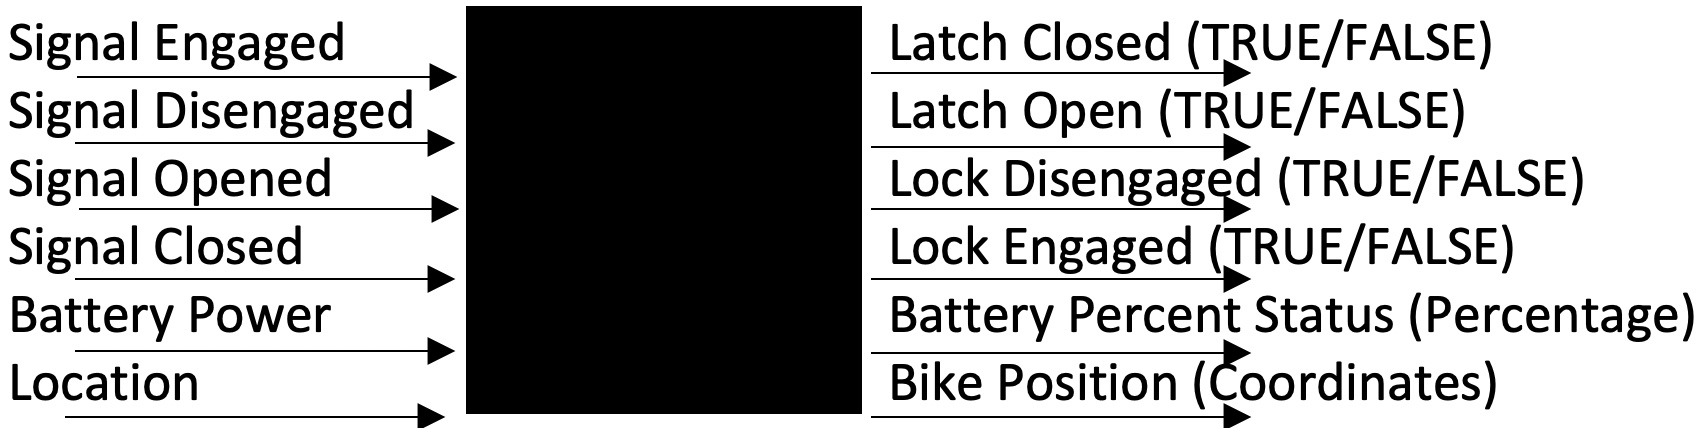
\includegraphics[width=0.6\linewidth]{./StimulusandResponses.jpeg}
 }
 \caption{\label{Stimulus and Responses} Stimulus and Responses}
 \end{center}
 \end{figure}
%%
\subsection{Notation}
~\newline
\begin{figure}[h!]
 \begin{center}
 {
 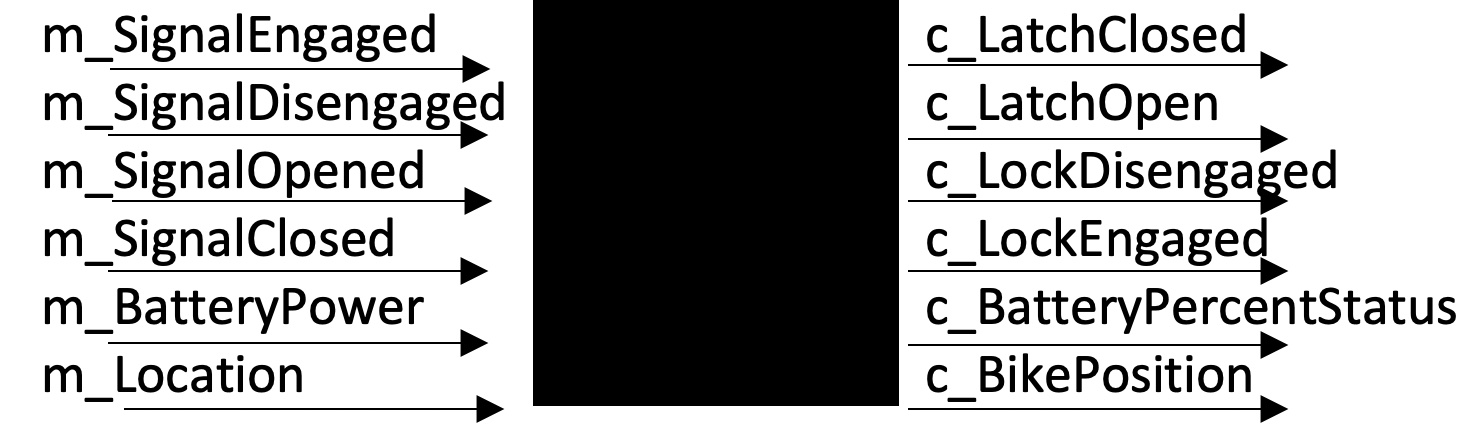
\includegraphics[width=0.6\linewidth]{./Notation.jpeg}
 }
 \caption{\label{Notation} Notation}
 \end{center}
 \end{figure}
%%
~\newpage
\subsection{Responses}
~\newline
\begin{figure}[h!]
 \begin{center}
 {
 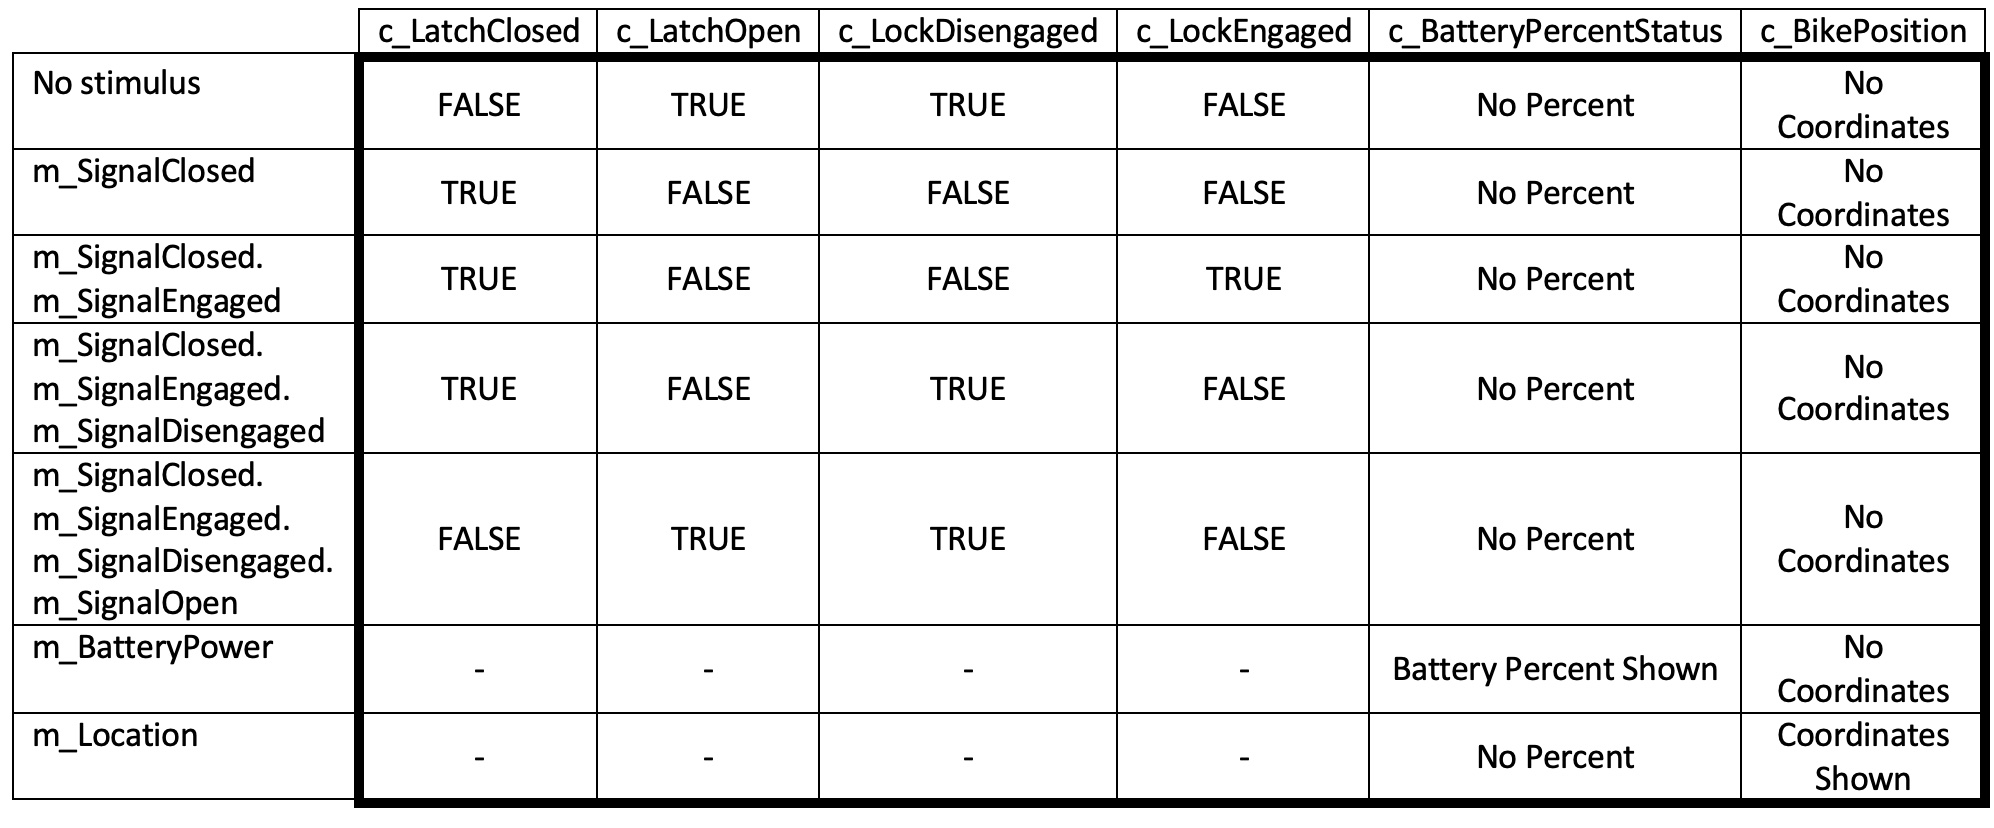
\includegraphics[width=0.9\linewidth]{./Responses.jpeg}
 }
 \caption{\label{Responses} Responses}
 \end{center}
 \end{figure}
%%
\subsection{Effect of Each Stimulus}
~\newline
\begin{figure}[h!]
 \begin{center}
 {
 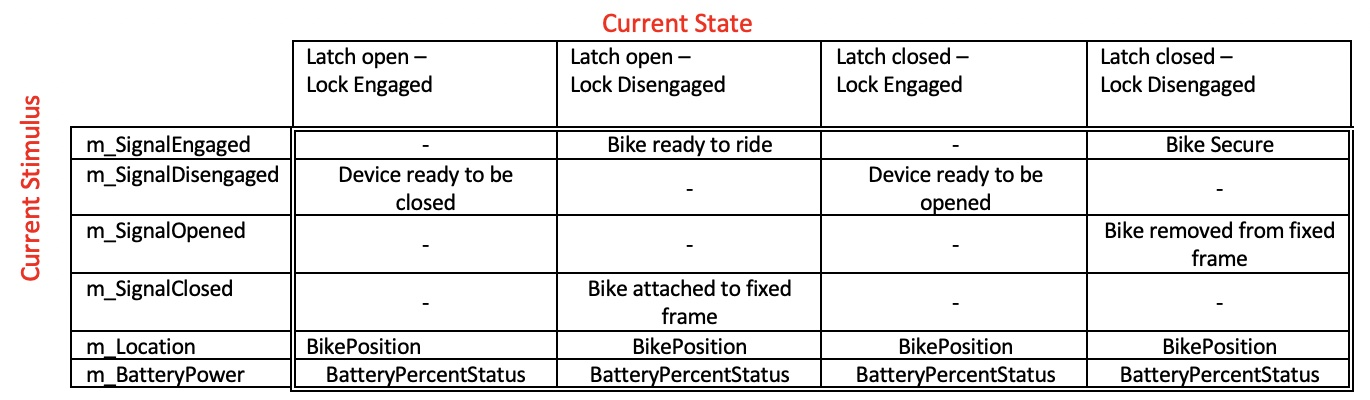
\includegraphics[width=0.9\linewidth]{./EffectofEachStimulus.jpeg}
 }
 \caption{\label{Effect of Each Stimulus} Effect of Each Stimulus}
 \end{center}
 \end{figure}
~\newpage
\section{Appendix B}
\subsection{Reflection}

The information in this section will be used to evaluate the team members on the
graduate attribute of Lifelong Learning.  Please answer the following questions:

\begin{enumerate}
  \item What knowledge and skills will the team collectively need to acquire to
  successfully complete this capstone project?  Examples of possible knowledge
  to acquire include domain specific knowledge from the domain of your
  application, or software engineering knowledge, mechatronics knowledge or
  computer science knowledge.  Skills may be related to technology, or writing,
  or presentation, or team management, etc.  You should look to identify at
  least one item for each team member.
  ~\newline
  ~\newline
 Steffi: 
  ~\newline
My lead role on this project is in regard to Documentation and Latex.  While I have experience with some project documentation, the extent to which it is necessary for this project is not something I have done before.  Looking at this project in such detail will help to more deeply understand every component of the project and help to better see the connection between every aspect.  Additionally, technical communication is a skill I have never used before so learning to use Github and Latex will be critical to the delivery of the project and developing skills that will be useful in future technical projects.
\\
\\
Abi:
\\
My lead role for this project is surrounding wireless communication, specifically Bluetooth.  I will need to learn how to implement Bluetooth communication between the SmartLock and the user's phone so that the lock can be disengaged remotely.  I have never worked with this type of technology before, so I will need to have a very steep learning curve. 
 \\
\\
Elsa:
\\ 
 I am the Embedded Systems Lead of the project, and as such I will be adding to my existing skills in order to design, build and provide support to other members of my team related to this topic. This project will require significant knowledge in the realm of electronics, wiring, microprocessor programming and general hardware systems. I am also a Support Lead of Documentation, which includes technical writing and typesetting in Latex. 
 \\
 \\
 Anthony: 
 \\
 The mobile application will be developed using XCode Ver.14.0, utilizing the Swift programming language for iOS Development. For linting, SwiftLint will be implemented as it is commonly used in the industry for iOS development utilizing XCode. Basic background in programming is a required skill needed to be able to effectively learn the IDE and programming language.
 I am the Embedded Systems Lead of the project, and as such I will be adding to my existing skills in order to design, build and provide support to other members of my team related to this topic.  This project will require significant knowledge in the realm of electronics, wiring, microprocessor programming and general hardware systems.  I am also a Support Lead of Documentation, which includes technical writing and typesetting in Latex. 
  \\
\\
Abdul:
\\ 
 Being on the app development sub-team, I will be required to acquire a working knowledge of the Swift programming language to develop the mobile application for the Smart Lock System.  In addition to that, I would need to research Bluetooth technology and its integration within our system.
 
 
  \item For each of the knowledge areas and skills identified in the previous
  question, what are at least two approaches to acquiring the knowledge or
  mastering the skill?  Of the identified approaches, which will each team
  member pursue, and why did they make this choice?
    ~\newline
    ~\newline
Steffi: 
  ~\newline
 Documentation - Two approaches that I can use to improve my skillset for documentation are reading old documentation that other groups have produced, or examples of documentation online, and writing documentation and paying careful attention to the focus of the section.  The emphasis will be placed on writing documentation because with this skillset I believe the best approach is to try and then learn from what was difficult and feedback on what was produced.  However, old documentation will still be referenced as well. 
  ~\newline
  Latex - Two approaches that can be used to improve my latex skill set are referencing external explanations (videos \& Tutorials), and trial and error with external reference materials.  I will be focusing on trial and error using some external materials.  I believe that seeing what happens for yourself when you make a change is the best way to understand what is going on.  The external resources will be used to give an idea of what it is possible to try to accomplish in latex, for example, certain formatting that I may not have considered existed. 
\\
\\
Abi:
\\ There are many different approaches to learning technical skills, such as Bluetooth.  I plan to approach learning this skill by researching on the Internet, asking our supervisor for potential resources or personal knowledge, seeking help from peers who have more knowledge on the subject.  After researching which hardware is needed to implement wireless communication, I will learn by doing, slowly building up my skills. Rather than choosing just one approach, I plan on using all of these approaches in parallel. 
\\
\\
Elsa:
\\ 
  I will acquire this expertise by learning through resources such as previous Embedded Systems and Electronics courses I have taken, online research and journals that I have access to through McMaster. Additionally, I find YouTube to be a useful experiential resource for learning how to apply acquired knowledge in personal projects. I will improve my technical writing and typesetting skills by practicing using Latex and challenging myself to continue researching and learning new modes of practice and editing.
\\
\\
Anthony:
\\
Apple has created their own modules to teach individuals how to use their IDE and programming language. Other resources include free YouTube tutorials and private companies offering courses. For the scope of this project and considering the complexity of the application, Apple’s free course and YouTube tutorials would be sufficient. Additionally, there are several public forums where individuals could search similar problems others have experienced before and find various solutions contributed by the community. Team member Anthony Shenouda has experience with the IDE as they have developed multiple mobile applications before. They will be responsible for the overall development and ensuring the application is completed successfully and timely. 
  
  I will acquire this expertise by learning through resources such as previous Embedded Systems and Electronics courses I have taken, online research and journals that I have access to through McMaster.  Additionally, I find YouTube to be a useful experiential resource for learning how to apply acquired knowledge in personal projects.  I will improve my technical writing and typesetting skills by practicing using Latex and challenging myself to continue researching and learning new modes of practice and editing.
\\
\\
Abdul:
\\ 
 Swift -  To learn Swift effectively, I plan to take a few starter courses as well as practise some basic programs using Swift. Doing so would familiarize myself with the Syntax and libraries. Most of the general programming basics I have already developed through my use of other languages. 
  
 Bluetooth - My approach to this would be to look at a few existing projects and adopt a similar approach within our system. Bluetooth is widely used, and there are a variety of open-source libraries of which we can take advantage.
\end{enumerate}

\end{document}